\documentclass[main.tex]{subfiles}
\begin{document}
\setcounter{section}{1}

\section{Installation and Getting Started}\label{sec:installation}

\subsection{Prerequisites}
Smooth Emulator software should run on UNIX, Mac OS or Linux, but is not supported for Windows OS. Smooth Emulator is largely  written in C++. In addition to a C++ compiler, the user needs the following software installed.

\begin{itemize}
    \item git
    \item CMake
    \item Eigen3 (Linear Algebra Package)
    \item GSL (Gnu Scientific Library)
    \item Python/Matplotlib (only for generating plots in the MCMC procedure)
\end{itemize}

CMake is an open-source, cross-platform build system that helps automate the process of compiling and linking for software projects. Hopefully, CMake will perform the needed gymnastics to find the Eigen3 and GSL installations. To install CMake, either visit the CMake website (https://cmake.org/), or use the system's package manager for the specific system. For example, on Mac OS, if one uses {\it homebrew} as a package manager, the command is\\
\vspace{-20pt}
{\tt 
\begin{verbatim} % brew install cmake\end{verbatim}
}

Eigen is a C++ template library for vector and matrix math, i.e. linear algebra. The user can visit the Eigen website (\url{https://eigen.tuxfamily.org/dox/}), or use their system's package manager. For example on Mac OS with {\it homeebrew},\\
\vspace{-20pt}
{\tt 
\begin{verbatim} % brew install eigen\end{verbatim}
}

The GNU Scientific Library (GSL) is a numerical library for C and C++ programmers. The library provides a wide range of mathematical routines such as random number generators, special functions and least-squares fitting. There are over 1000 functions in total with an extensive test suite. One can either download the software from the GSL website (https://www.gnu.org/software/gsl/), or use a package manager. Again, for {\it homebrew} on Mac OS,\\
\vspace{-20pt}
{\tt 
\begin{verbatim} % brew install gsl\end{verbatim}
}

\subsection{Making Home Directory and Setting Home Environment Variable}

The software requires two repositories. They should be cloned into the same directory. For compilation purposes this directory needs to be accessed via an environmental variable.  For example the directory might be named {\tt githome\_msu} (another name would be fine, just substitute it everywhere below). First, create the directory, then enter that directory,\\
\vspace{-20pt}
{\tt 
\begin{verbatim}
    % mkdir (some path)/githome_msu
    % cd (some path)/githome_msu
\end{verbatim}
}
Here, ``(some path)'' might be something like {\tt /Users/CarlosSmith}. Then, create an environmental variable which describes the location of the directory above.\\
\vspace{-20pt}
{\tt 
\begin{verbatim}
    % export GITHOME_MSU=(some path)/githome_msu
\end{verbatim}
}
It is recommended to copy this command into the user's {\tt .bashrc} (or equivalent) file to avoid re-defining it each time one needs to recompile.

\subsection{Downloading}\label{sec:Downloading_Compiling}
From within the {\tt githome\_msu/} directory,\\
\vspace{-20pt}
{\tt 
\begin{verbatim}
    % git clone https://github.com/scottedwardpratt/smooth.git
    % git clone https://github.com/scottedwardpratt/commonutils.git
\end{verbatim}
}

This creates 2 directories: {\tt .../githome\_msu/commonutils} and {\tt .../githome\_msu/smooth}.

\subsection{Directory and File Structure}

The directory structure of the repository is as follows: 

\centerline{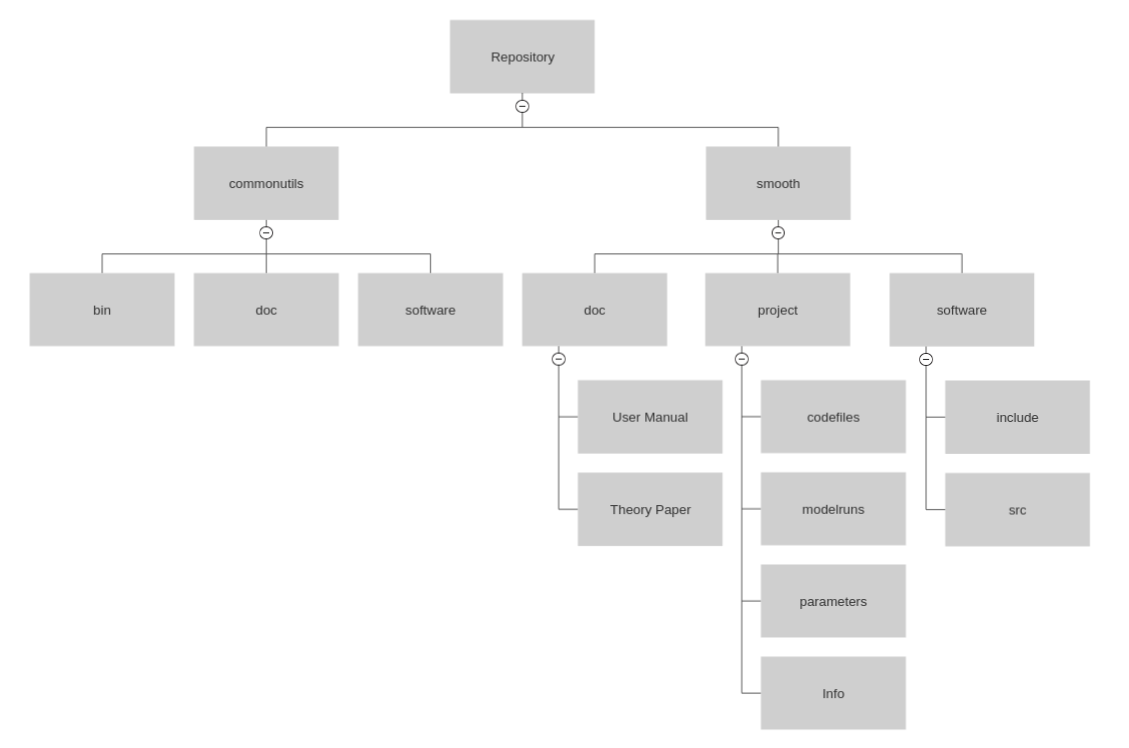
\includegraphics[width = 0.95\textwidth]{Structure_Tree.png}}

Once compiled, the material in the {\tt commonutils/} directory creates a library that is used for a variety of tasks, not particularly designed for Smooth Emulator or Simplex Sampler. The {\tt smooth/} directory contains codes that are used to create libraries specific to the sampler and emulator. The {\tt smooth} directory also includes a {\tt smooth/local/} directory. Executables are stored in {\tt smooth/local/bin}. The short main program source files are located in {\tt smooth/local/main\_programs/}. It is not envisioned that the User would edit files in the {\tt smooth/software/} directory, but that the User may well wish to create custom versions of the short main programs in {\tt smooth/local/main\_programs/}.

\subsection{Compiling Libraries }

First, change into software directories, then create the makefiles with cmake, then compile them.\\
\vspace{-20pt}
{\tt 
\begin{verbatim}
    % cd ../githome_msu/smooth/commonutils/software
    % cmake .
    % make
    % cd ../githome_msu/smooth/software
    % cmake .
    % make
\end{verbatim}
At this point all the libraries are built. Finally, compile the main programs. Below, this illustrates how to build the programs used for generating training points with Simplex and for tuning the emulator with Smoothy:
\begin{verbatim}
    % cd ../githome_msu/smooth/local/build
    % cmake .
    % make simplex
    % make smoothy_writecoefficients
    % make smoothy_readcoefficients
\end{verbatim}
}
Other main programs can also be found in {\tt ../githome\_msu/smooth/local/main\_programs}. If you build your own main programs (probably using these as examples), you can edit the {\tt CMakeList.txt} file in {\tt ../githome\_msu/smooth/local/build} as an example. The executables should appear in {\tt ../githome\_msu/smooth/local/bin/}. 

\subsection{Making a Project Directory}

Create a directory anywhere on your computer and copy the template directory.
{\tt 
\begin{verbatim}
    % cp -r ../githome_msu/smooth/project_template my_project
\end{verbatim}
}
Within {\tt my\_project/} there are three sub-directories. The first is {\tt my\_project/Info/}. Information about the model parameters, and their priors is stored in {\tt my\_project/prior\_info.txt}, and information about the observables is store in {\tt my\_project/observable\_info.txt}. The {\tt my\_project/parameters} directory stores user-defined parameter files used by Simplex Sampler, {\tt my\_project/parameters/simplex\_parameters.txt}, and by Smooth Emulator {\tt my\_project/parameters/emulator\_parameters.txt}. The {\tt my\_project/modelruns} directory will store information for each full-model run. The directories
{\tt  my\_project/modelruns/run0/}, {\tt  my\_project/modelruns/run1/}, $\cdots$, have files describing the model parameters for each run, along with the output required by the emulator for each specific full-model run. For example, the {\tt  my\_project/modelruns/run1/} directory has the files {\tt mod\_parameters.txt} and {\tt obs.txt}. The first file stores the model parameter values for that particular training run. The User then runs their full model based on those parameters and stores the corresponding observables in {\tt obs.txt}. The User may generate the {\tt mod\_parameters.txt} files using Simplex Sampler, or the user might generate them according to some other prescription. Once the User has then generated the {\tt obs.txt} files, Smooth Emulator can then build and tune the emulator.

\end{document}
